\documentclass[11pt,wide]{article}

\usepackage{graphicx}
%\usepackage{caption}
\usepackage{subcaption}
\usepackage{float}
%\usepackage{epstopdf}

\usepackage{amsmath,amssymb,amsfonts,amsthm,mathtools}

\usepackage{bbm}
\usepackage{hyperref}
\usepackage{url}
\usepackage[T1]{fontenc}
\usepackage[polish]{babel}
\usepackage{comment}      

\usepackage{csvsimple}
\usepackage[section]{placeins}

\newtheorem{definition}{Definicja}[section]

\title{\LARGE\textbf{Pracownia 1 z analizy numerycznej}\\Zadanie 15}
\author{Krzysztof Wasielewski 322091}
\date{Listopad 2021}

\begin{document}

\maketitle

\section{Wstęp}

Interpolacja to zadanie polegające na skonstuowaniu funkcji na podstawie wartości funkcji w węzłach. Istnieje szereg metod, które pozwalają na efektywne wykorzystanie ograniczonej informacji o interpolowanej funkcji. Szerzej omówiona zostanie interpolacja za pomocą \textit{okresowej funkcji sklejanej III stopnia}.

\subsection{Funkcje sklejane}
\theoremstyle{definition}

\begin{definition}
Dla danych $n$, $n\in\mathbb{N}$, węzłów $x_0, x_1, \dots, x_n$ ($x_0 = a < x_1 < \dots < x_n = b$) oraz funkcji $f$ funkcją sklejaną interpolacyjną k-tego stopnia nazywamy funkcję $s$, taką że:
\begin{enumerate}
    \item w każdym z przedziałów $[x_{i-1}, x_i](i = 1, 2,\dots, n)$ funkcja $s$ jest wielomianem stopnia co najwyżej $k$
    \item $s(x_i) = f(x_i)$ $(i = 0, 1,\dots, n)$
    \item funkcja $s$ ma pochodne rzędu $0, 1, \dots, k-1$ ciagłe na przedziale $[a, b]$
\end{enumerate}
Dodatkowo funkcja $s$ jest nazywana okresową, gdy $f(x_n) = f(x_0)$ oraz $s^{(i)}(a+0)=s^{(i)}(b-0)$ $(i = 0, 1, \dots k-1)$
\end{definition}
Dla uproszczenia zapisu niech $s_i$ oznacza $s\rvert_{[x_i, x_{i+1}]}$.

Skonstruowanie funkcji sklejanej $s$ polega na dobraniu współczynników kolejnych wielomianów, składających się na tę funcję. Odpowiednie ich dostrojenie sprawia, że funkcja $s$ jest regularna tj. $s \in C^k [a,b]$. 

Funkcja sklejana interpolacyjna III stopnia opisana jest jednoznacznie przez $4n$ współczynników. Należy zatem znaleźć tyle samo warunków, pozwalających na rozwiązanie problemu. Pierwsze $2n$ warunków pochodzi z~analizy równości $s_{i} (x_{i+1})= f(x_{i+1}) = s_{i+1} (x_{i+1})$. Kolejne $2n-2$ warunków pochodzi z równości $s_i^{(1)}(x_{i+1})=s_{i+1}^{(1)}(x_{i+1})$ oraz $s_i^{(2)}(x_{i+1})=s_{i+1}^{(2)}(x_{i+1})$, czyli przyrównania do siebie pochodnych pierwszego i drugiego rzędu sąsiednich wielomianów. Pozostałe dwa warunki, których wyprowadzenie nie jest tak jasne jak pozostałych, zostanie przedstawione w osobnym fragmencie sprawozdania, które referuje pełne wyprowadzenie obliczeń. 

\subsection{Krzywe parametryczne}
Krzywe parametryczne jednego parametru są określane przez układy równań uzależnionych od parametru. Przykładowo równanie parametryczne dla okręgu o środku $S(0,0)$ i promieniu $R$ dla parametru $t$ wygląda następująco:
\begin{equation}
    \begin{cases}
    x = R \cos(t)\\
    y = R \sin(t)
    \end{cases}
\end{equation}

\subsection{Cel zadania}

Dla zadanej zamkniętej krzywej parametrycznej ($x=x(t)$, $y=y(t)$) należy skonstruować zamkniętą krzywą sklejaną interpolacyjną, przez wyznaczenie funkcji sklejanych interpolujących III stopnia $s_x(t)$, $s_y(t)$, takich że znaleziona krzywa ma przedstawienie $x=s_x(t)$, $y=s_y(t)$. Węzły, na podstawie których wyznaczone zostaną funkcje $s_x$ oraz $s_y$, wybrane zostaną z dziedziny parametru t (próbka lub ustalony podzbiór np. równoodległych liczb)

\section{Wyznaczanie funkcji sklejanej}
\subsection{Wyprowadzenie układu warunków}
%TODO sprawdzić indeksowanie
Do wyznaczenia parametrów krzywej sklejanej potrzebne jest wyznaczenie współczynników dla każdego $s_i$. Niech $h_i = x_{i+1}-x_i$, $s_i^{(2)}(x_i)=z_i$ oraz $s_{i}^{(2)}(x_{i+1})=z_{i+1}$. Ponieważ $s_i$ jest wielomianem stopnia co najwyżej 3 to $s_i^{(2)}$ jest funkcją liniową, dlatego
$$s_i^{(2)}(x) = \frac{z_i}{h_i}(x_{i+1}-x)+\frac{z_{i+1}}{h_i}(x-x_i)$$
Chcąc otrzymać współczynniki $s_i$ powyższe równanie należy dwukrotnie scałkować.
$$s_i(x) = \frac{z_i}{6h_i}(x_{i+1}-x)^3+\frac{z_{i+1}}{6h_i}(x-x_i)^3+a(x-x_i)+b(x_{i+1}-x)$$
gdzie a i b są stałymi całkowania. Wyznaczyć je można z wartości w węzłach interpolacyjnych. Ponieważ zachodzi $s_i(x_i)=y_i$ oraz $s_i(x_{i+1})=y_{i+1}$ otrzymujemy
$$s_i(x)=\frac{z_i}{6h_i}(x_{i+1}-x)^3+\frac{z_{i+1}}{6h_i}(x-x_i)^3+(\frac{y_{i+1}}{h_i}-\frac{z_{i+1}h_i}{6})(x-x_i)+(\frac{y_{i}}{h_i}-\frac{z_{i}h_i}{6})(x_{i+1}-x)$$
Różniczkując powyższe równanie i ewaluując je dla $x=x_i$
$$s_i^{(1)}(x_i)=-\frac{h_i}{3}z_i-\frac{h_i}{6}z_{i+1}-\frac{y_i}{h_i}+\frac{y_{i+1}}{h_i}$$
Analogicznie dla $s_{i-1}$
$$s_{i-1}^{(1)}(x_i)=-\frac{h_{i-1}}{3}z_{i-1}-\frac{h_{i-1}}{6}z_{i}-\frac{y_{i-1}}{h_{i-1}}+\frac{y_{i}}{h_{i-1}}$$
Ponieważ $s_{i-1}^{(1)}(x_i)=s_{i}^{(1)}(x_i)$
$$h_{i-1}z_{i-1}+2(h_{i-1}+h_i)+h_iz_{i+1}=\frac{6}{h_i}(y_{i+1}-y_i)-\frac{6}{h_{i-1}}(y_i-y_{i-1})$$  dla i takiego że $1\leq i\leq n$, gdzie $h_0=h_n$
Do znalezienia $z_i$ przydatna staje się notacja macierzowa układu równań
\begin{equation}
\begin{split}
\begin{bmatrix}
    2(h_0+h_1) & h_1 & &\dots& & h_0\\
    h_1 & 2(h_1+h_2) & h_2&&& \\
    \vdots& && \ddots && \\
    & &&h_{n-1} &2(h_{n-1}+h_n) & h_n\\
    h_n& & &&h_{n-1} & 2(h_{n-1}+h_{n}) \\
\end{bmatrix}
\begin{bmatrix}
z_1\\
\\
\\
\\
z_n\\
\end{bmatrix}
\\=
\begin{bmatrix}
\frac{6}{h_1}(y_2-y_1)-\frac{6}{h_0}(y_1-y_0)\\
\\
\\
\\
\frac{6}{h_n}(y_1-y_n)-\frac{6}{h_{n-1}}(y_n-y_{n-1})\\
\end{bmatrix}
\end{split}
\end{equation}

Do rozwiązania takiego układu można wykorzystać np. eliminację Gaussa. Współczynnik $z_0$ otrzymujemy z równości $z_0 = z_n$. Po wyznaczeniu $z_i$ funkcja $s_i$ prezentuje się natępująco
\begin{equation}
\begin{split}
    s_i(x)= y_i + (x-t_i)\Big(-\frac{h_i}{6}(z_{i+1}+2z_i)+\frac{1}{h_i}(y_{i+1}-y_i)\\+(x-y_i)\big(\frac{z_i}{2}+\frac{1}{6h_i}(x-t_i)(z_{i+1}-z_i)\big)\Big)
\end{split}
\end{equation}


\subsection{Wyznaczanie zamkniętej krzywej sklejanej}
Znając metodę wyznaczania okresowej funkcji sklejanej, można przystąpić do skonstruowania zamkniętej krzywej sklejanej interpolacyjnej. Ponieważ krzywe w tym zadaniu są dwuwymiarowe to potrzebne będą dwie funkcje sklejane. Każda z nich będzie uzależniała jedną ze współrzędnych od parametru $t$. Ciąg węzłów $t_0, t_1, \dots, t_n$ musi spełniać warunek $a \leq t_i < t_{i+1} \leq b$. Ponieważ końcami przedziału $a$ i $b$ można manipulować, nic nie stoi na przeszkodzie, by założyć dodatkowo, że $t_i + 1 = t_{i+1}$. Wówczas równanie $(2)$ przyjmuje postać
\begin{equation}
\begin{split}
\frac{1}{6}
\begin{bmatrix}
    4 & 1 & &\dots& & 1\\
    1 & 4 & 1&&& \\
    \vdots& && \ddots && \\
    & &&1 &4 &1\\
    1& & &&1 & 4 \\
\end{bmatrix}
\begin{bmatrix}
z_1\\
\\
\\
\\
z_n\\
\end{bmatrix}
=
\begin{bmatrix}
y_2+y_0-2y_1\\
\\
\\
\\
y_1+y_{n-1}-2y_n\\
\end{bmatrix}
\end{split}
\end{equation}
co upraszcza implementację. Po wyznaczeniu funkcji sklejanych $s_x$, $s_y$ zmodyfikowaną metodą poszukiwane krzywe można wyrysować, wyliczając
punkty $(s_x(t), s_y(t))$ dla $t \in [a, b]$.
Zauważmy, że macierz w $(3)$ jest macierzą cykliczną. Rozwiązanie układu w postaci $Cx=y$, gdzie C jest macierzą cykliczną można otrzymać w następujący sposób: $C$ jest macierzą diagonalizowalną przez znormalizowaną macierz Fouriera, czyli $C=Fdiag(\lambda_1, \dots, \lambda_n)F^{-1}$, gdzie $\lambda_i$ jest wartością własną macierzy C. Obliczanie odwrotności macierzy Fouriera można zastąpić przez policzenie $F^*$, gdzie operator $*$ oznacza sprzężenie hermitowskie. Wówczas zachodzi $C=Fdiag(\lambda_1, \dots, \lambda_n)F^*$. Rozwiązanie układu ma zatem postać $x = Fdiag(\lambda_1^{-1}, \dots, \lambda_n^{-1})F^*y$.
\\

\section{Część obliczeniowa}
Poznawszy sposób wyznaczania krzywych sklejanych interpolacyjnych, można przystąpić do zastosowania jej w przykładach.
\subsection{Okrąg}
Do zadania wybrany został okrąg o przedstawieniu parametrycznym
\begin{equation}
    \begin{cases}
    x = \cos(\frac{\pi}{10} t)\\
    y = \sin(\frac{\pi}{10} t)
    \end{cases}
\end{equation}
\begin{figure}[!htb]
    \centering
    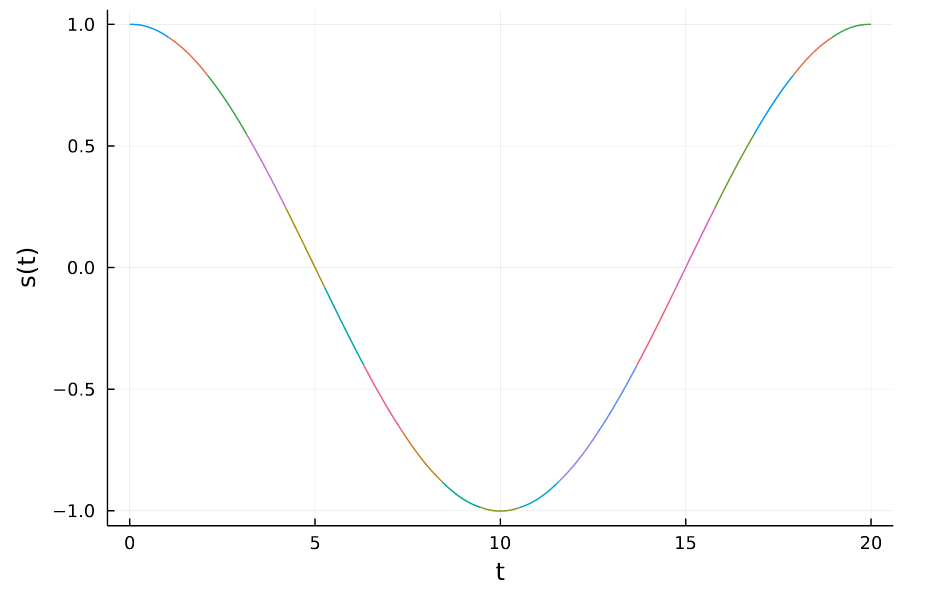
\includegraphics[width=120mm]{okragsx.png}
    \caption{Funkcja sklejana interpolująca $cos(\frac{\pi}{10}t)$}
    \label{fig:my_label}
\end{figure}
\begin{figure}[!htb]
    \centering
    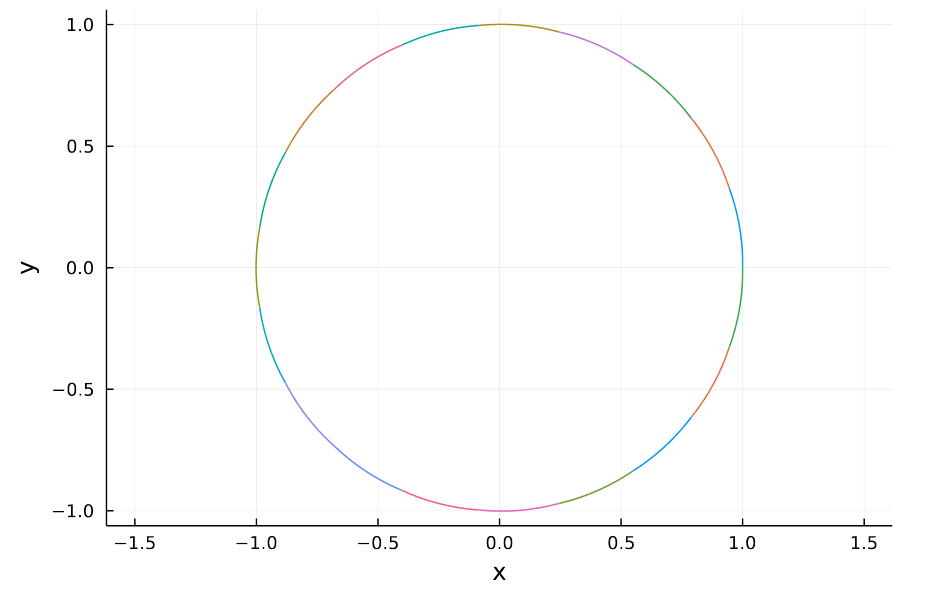
\includegraphics[width=120mm]{okrag.png}
    \caption{Krzywa sklejana interpolująca okrąg}
    \label{fig:my_label}
\end{figure}
Kolejne przedziały $[t_i, t_{i+1}]$ zaznaczone są na rysunkach osobnym kolorem. Dzięki zastosowaniu okresowej funkcji sklejanej otrzymujemy efekt wizualnej gładkości funkcji (rozumianej nieformalnie, a nie jako relacja $f \in C^\infty$) nawet na końcach przedziału. Gdyby zastosować naturalną funkcję sklejaną do interpolacji krzywej zamkniętej to miejsce zapętlania się krzywej byłoby łatwo rozpoznawalne, bo pierwsze pochodne $s_0$ i $s_n$ w punkcie $t_n=t_0$ nie zawsze byłyby równe, przez co powstawałby tam ostry kant.
\begin{figure}[!htb]
    \centering
    \includegraphics[width=120mm]{okragnatural.png}
    \caption{Okrąg z widocznym błędem w otoczeniu punktu (1, 0) }
    \label{fig:my_label}
\end{figure}
\subsection{Elipsa}
Wybrana elipsa
\begin{equation}
    \begin{cases}
    x = 3\cos(\frac{\pi}{10} t)\\
    y = \frac{1}{2}\sin(\frac{\pi}{10} t)
    \end{cases}
\end{equation}
\begin{figure}[H]
    \centering
    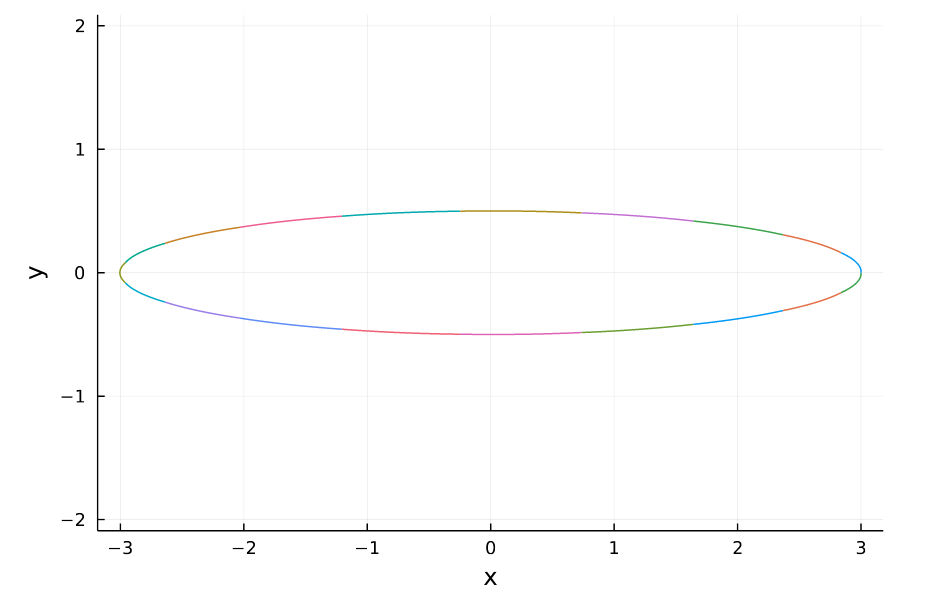
\includegraphics[width=120mm]{elipsa.png}
    \caption{Krzywa sklejana interpolująca elipsę}
    \label{fig:my_label}
\end{figure}
\subsection{Tajemnicza krzywa}
\begin{figure}[H]
    \centering
    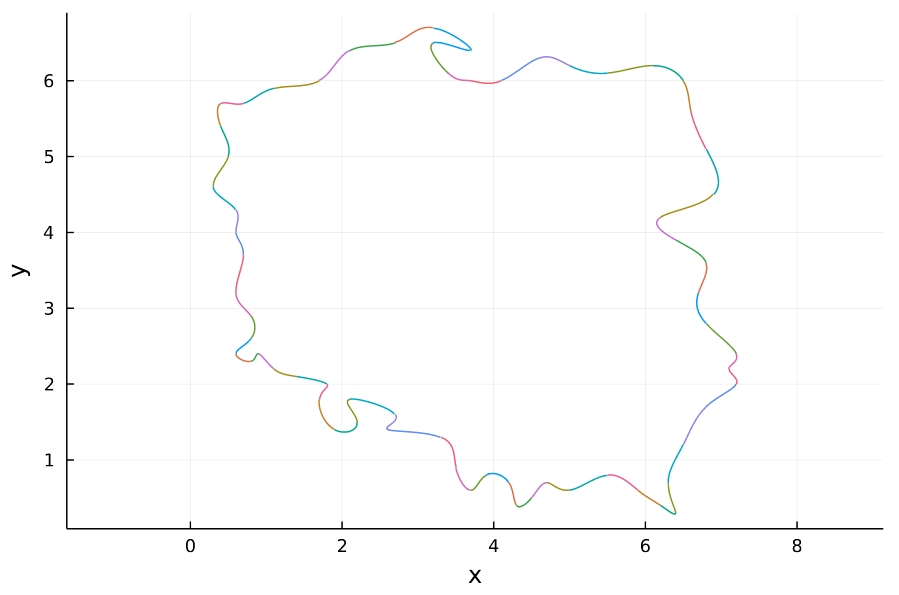
\includegraphics[width=120mm]{tajemnicza.png}
    \caption{Krzywa intepolująca granice Polski}
    \label{fig:my_label}
\end{figure}
\subsection{Epitrochoida}
Epitrochoida to krzywa parametryczna opisana układem równań
\begin{equation}
    \begin{cases}
    x = (R+r)\cos(t)-h \cos(\frac{R+r}{r}t)\\
    y = (R+r)\sin(t)-h \sin(\frac{R+r}{r}t)
    \end{cases}
\end{equation}
Jeśli $\frac{R}{r}$ jest liczbą wymierną to epitrochoida jest krzywą zamkniętą. Epitrochoida w tym zadaniu
\begin{equation}
    \begin{cases}
    x = 7\cos(\frac{\pi}{20}t)-3 \cos(\frac{7}{2}\frac{\pi}{20}t)\\
    y = 7\sin(\frac{\pi}{20}t)-3 \sin(\frac{7}{2}\frac{\pi}{20}t)
    \end{cases}
\end{equation}
\begin{figure}[H]
    \centering
    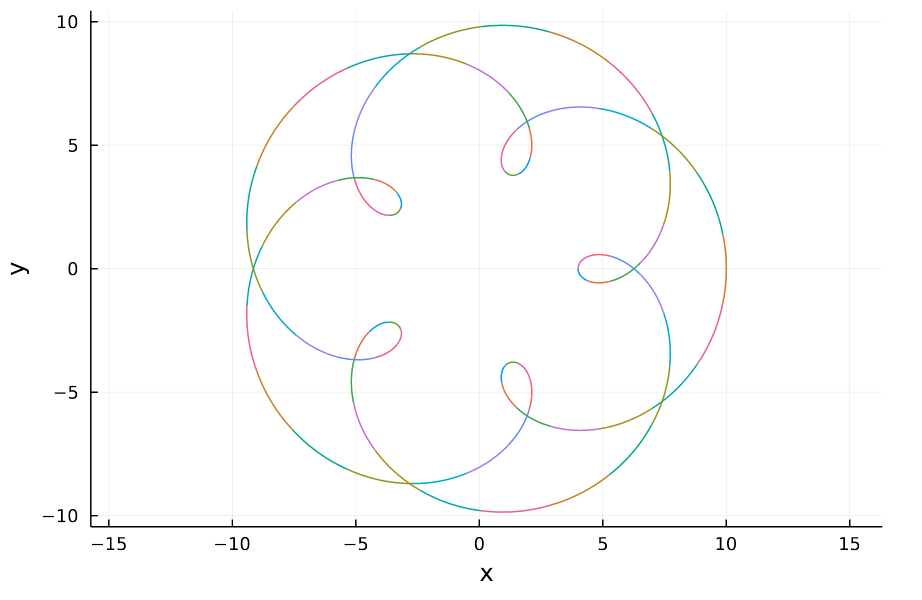
\includegraphics[width=120mm]{epitrochoid.png}
    \caption{Przykładowa epitrochoida}
    \label{fig:my_label}
\end{figure}
\subsection{Oszacowanie błędu}
Do wykazania skuteczności metody obliczono pierwiastek z błędu średniokwadratowego, który ilustruje średnią odległość punktów na krzywej sklejanej od punktów wyliczonych z równań parametrycznych. Obliczenia wykonano w formatach Float64 i Complex64\\
\begin{center}
\begin{tabular}{|l|c|c|c|}
\hline
     & okrąg & elipsa & epitrochoida\\ \hline
     RMSE & 0.0010 & 0.0022 & 0.0017 \\\hline
\end{tabular}
\end{center}
\section{Podsumowanie}
Okresowość funkcji sklejanej w prosty sposób przekłada się na stosowalność tej metody interpolacji w przybliżaniu zamkniętych krzywych parametrycznych. Podobnie jak w przypadku naturalnych funkcji sklejanych, okresowe funkcje sklejane pozbywają się efektu Rungego, kosztem większej liczby parametrów do zapamiętania. Zastosowanie równoodległych węzłów parametru pozwala na zredukowanie złożoności obliczeniowej, wynikającej z rozwiązywania układu (2) eliminacją Gaussa, przez wykorzystanie macierzy Fouriera. 
%%%%%%%%
\begin{thebibliography}{}

\bibitem{texbook}David Kincaid, Ward Cheney (1991) Numerical Analysis: Mathematics of Scientific Computing
\bibitem{texbook}Mingkui Chen (1987) On the Solution of Circulant Linear Systems
\bibitem{texbook}Hans-Peter Moser (dostęp 19.11.2021) Periodic splines\\ http://www.mosismath.com/PeriodicSplines/PeriodicSplines.html

\end{thebibliography}
\end{document}


